Bereits in \autoref{sec:mot} wurde gezeigt, dass das Problem der gravitationellen Wechselwirkungen in unserer Galaxie mit einem aktuellen Computer nicht ohne 
    weiteres lösbar ist. 
    Konnten sich früher Programmierer darauf verlassen, dass in einigen Jahren eine deutlich schnellere Prozessorgeneration erscheinen würde, so dass Probleme ohne 
    weitere Änderungen schneller gelöst werden könnten, ist dies heute leider nicht mehr der Fall. 
    
    Grund hierfür ist die Physik. Dazu ein kleines Rechenexperiment: Nehmen wir einen Prozessorchip von etwa einem Zentimeter Durchmesser an und vergegenwärtigen wir 
    uns die Lichtgeschwindigkeit $c \approx 3\cdot10^{10}$ \footnote{Bureau International des Poids et Mesures [1975], \textit{Resolution 2 of the 15th CGPM},\\URL:
    https://www.bipm.org/en/CGPM/db/15/2/ Abgerufen am 16.07.2018}. Licht könnte diesen Chip also etwa 30 Milliarden mal pro Sekunde durchqueren, was 30 Gigahertz
    entspräche. Bedenkt man, dass man in Prozessoren mit Elektrizität arbeitet und somit beispielsweise mit kapazitären Effekten und proportional zur Taktfrequenz steigender
    Verlustleistung zu kämpfen hat, sind die 3 Gigahertz aktueller Mittelklasseprozessoren durchaus nicht zu verachten.
    
    Zwar wäre eine Möglichkeit die Chips weiter zu verkleinern, jedoch machen dem Fortschritt hier quantenmechanische Phänomene aktuell noch einen Strich durch die Rechnung.
    Ein gängiger und gangbarer Lösungsweg besteht in der Parallelisierung von Soft- und Hardware. Durch das gleichmäßige verteilen eines Algorithmus auf mehrere Prozessoren
    kann die Gesamtlaufzeit entsprechend verringert werden. Unter optimalen Bedingungen könnte theoretisch eine Verdopplung der Prozessoranzahl eine Halbierung der Laufzeit
    bewirken. Heute haben daher die meisten Prozessoren nicht mehr nur einen Rechenkern, sondern mehrere und für die Berechnung großer mathematischer Probleme arbeiten oft viele
    Rechner zusammen an der Lösung. \citep{hpcskript}
    
    Ein weiterer Grund für parallele, beziehungsweise verteilte Rechnersysteme ist die Diskrepanz zwischen vorhandenem und benötigtem Speicher. Beispielsweise hat der diesbezüglich größte
    Computer im Rechenzentrum der Christian-Albrecht-Universität Kiel einen Hauptspeicher von 768 GB. Ein aktuelles, speicherintensives Problem ist ein engmaschiges 
    Klimamodell der Erde. Bei einer Dichte von einer Masche alle 1,56 km in Äquatornähe wird der Gesamtspeicherbedarf auf etwa 24000 GB geschätzt \citep{climate}. Ein Problem
    dieser Größe passt nicht mehr in den Hauptspeicher eines Computers.
    Hinzu kommt die Skalierbarkeit solcher Probleme: Angenommen ein Hauptspeicher von 24000 GB stünde auf einem Computer zur Verfügung. Warum bei einer Maschendichte von 
    1,56 km stehen bleiben und nicht noch feiner auflösen um noch genauere Berechnungen durchzuführen?
    Warum bei der Berechnung der gravitationellen Wechselwirkungen bei den Sonnen unserer Galaxie stehen bleiben und nicht die Planeten, Monde oder noch kleinere Himmelskörper mit einbeziehen? 
    Diese Probleme, und damit auch der Speicherbedarf, lassen sich also nahezu beliebig vergrößern.
    
    Im folgenden Kapitel wird kurz skizziert, wie parallel arbeitende Hardware gestaltet sein kann und welche Vor- und Nachteile und welche Herausforderungen damit einhergehen. Grundbegriffe
    der Computerarchitektur werden vorausgesetzt, da eine Einführung den Umfang dieser Arbeit sprengen würde.
    
    \subsection{Parallele Hardware}
    \label{sec:parhard}
      \subsubsection{Prozessor}
      \label{sec:processor}
      \citet{flynn} klassifiziert 4 unterschiedliche Architekturen von Rechnern. Dabei unterteilt er nach der Möglichkeit des Prozessors zu einem Zeitpunkt einzelne oder mehrere
      Instruktionen beziehungsweise Datensätze zu verarbeiten (vgl. \autoref{tab:flynn}).
      \begin{table}[tb]
	\centering
	\begin{tabular}{|p{3.5cm}|p{4cm}|p{4cm}|}
	  \hline
			                             & eine Instruktion \newline (single instruction)       & mehrere Instruktionen \newline (multiple instruction) \\
	  \hline
	  ein Datensatz \newline (single data)       & SISD: konventioneller \newline einkerniger Prozessor & MISD: Spezialrechner                                  \\
	  \hline
	  mehrere Datensätze \newline (multiple data)& SIMD: Vektorrechner                                  & MIMD: Multicore; \newline Clustersystem               \\
	  \hline
	\end{tabular}
	\caption{Flynnsche Klassifikation mit Beispielen.}
	\label{tab:flynn}
      \end{table}
      
      Vor einigen Jahrzehnten waren die meisten Prozessoren in PCs noch SISD-Architekturen. Sie hatten einen Prozessor mit einem einzelnen Kern; konnten also zu jedem Zeitpunkt nur eine Instruktion
      auf einem Datensatz ausführen. Heute sind Multicore-Prozessoren üblich. Auf einem Prozessorchip finden sich hierbei mehrere Rechenkerne. Die einzelnen Kerne sind unabhängig von einander; sie 
      verwalten eigene Register und führen eigene Instruktionen aus. Daher zählen Multicore-Prozessoren zu den MIMD-Architekturen. Zu diesen Architekturen gehören ebenfalls die später erläuterten 
      \hyperref[sec:netzwerk]{Clustersysteme}. \citep{flynn, multicore}
      
      MIMD-Architekturen sind auf Grund ihrer autonom arbeitenden und programmierbaren Prozessoren sehr flexibel und können viele Probleme effizient lösen. Die Autonomie der Prozessoren
      stellt die Programmierung aber auch vor Herausforderungen. Durch die asynchrone Ausführung der Programme wird das Verhalten des gesamten Systems schwer vorhersagbar. \citep{hpcskript}
      
      MISD-Architekturen, also solche in denen parallel auf einem Datum mehrere Instruktionen ausgeführt werden können, sind nur in Spezialrechnern zu finden und für die Lösung der meisten
      Probleme nicht geeignet. \citep{architect, korbler}
      
      SIMD-Architekturen hingegen, in denen auf mehreren Daten parallel die gleiche Instruktion ausgeführt werden kann, sind durchaus gängig.
      Hintergrund sind Algorithmen, die auf ganzen Reihen von Daten immer wieder die selbe Operation ausführen. Während beim Ansatz der MIMD-Architekturen die Operationen dynamisch auf die
      einzelnen Recheneinheiten verteilt werden, ist der Ansatz von SIMD-Architekturen, beziehungsweise von Vektorrechnern, die Anzahl der Rechenwerke in den Recheneinheiten zu erhöhen 
      und eine Operation für mehrere Daten gleichzeitig auszuführen. Zum Beispiel werden für die Berechnung der Gravitationskräfte für viele Körper immer wieder die selben Operationen 
      verarbeitet. Anstatt diese also für jedes einzelne Paar von Körpern durchzuführen, könnten sie für mehrere Paare von Körpern gleichzeitig durchgeführt werden.
      
      Der Name Vektorrechner leitet sich von der Anlehnung an die kartesische Geometrie her, in der ein Vektor ein Tupel von Zahlen ist. Entsprechend werden Daten des selben Typs ebenfalls 
      als Vektoren bezeichnet. Um solche Vektoren handhaben zu können, verfügen Vektorrechner über spezielle Vektorregister, die mehrere Daten gleichzeitig fassen können. Für jedes einzelne
      Datum innerhalb dieser Register ist dann jeweils ein eigenes Rechenwerk im Kern zuständig. \citep{hpcskript}
      
      Prozessoren laden in der Regel nicht nur ein einzelnes Datum, sondern gleich eine sogenannte \textit{cache line} aus dem Hauptspeicher. Daher ist es sinnvoll, 
      um SIMD-Parallelisierung optimal ausnutzen zu können, die Daten im Hauptspeicher anhand dieser cache lines anzuordnen. Dazu müssen in der Regel explizite Methoden zum Anfordern von 
      \wlabel{\textit{aligned memory}}{w:aligned} verwendet werden. Außerdem müssen die parallel zu verarbeitenden Daten im Hauptspeicher direkt hintereinander und nicht durch andere Daten 
      unterbrochen auftauchen. Nehmen wir an, wir wollten die Daten der Körper, die für die Berechnung der Gravitationskräfte benötigt werden, in einer Struktur zusammenfassen. Wollen wir
      Daten zu vielen dieser Körper speichern so wäre es in Bezug auf Vektorrechner nicht sinnvoll ein Array dieser Strukturen anzulegen (engl.: \wlabel{\textit{array of structs}}{w:aos}).
      Dabei würden die im Sinne der Vektorisierung zusammengehörigen Daten durch andere getrennt. Um eine Vektorisierung zu ermöglichen ist es daher sinnvoll die Struktur so zu definieren,
      dass sie Arrays der benötigten Daten beinhaltet (engl.: \wlabel{\textit{struct of arrays}}{w:soa}). So kann sichergestellt werden, dass diese Daten im Hauptspeicher hintereinander stehen.
      \citep{hpcskript, architect}
      
      Viele aktuelle Multicore-Prozessoren verfügen zusätzlich über einige Möglichkeiten der Vektorisierung. Es existieren aber auch auf diese Art der Parallelisierung spezialisierte Prozessoren.
      \citep{architect}
      
      \subsubsection{Speicherverwaltung}
      \label{sec:speicher}
	In \autoref{sec:parrech} wurde bereits kurz erwähnt, dass bei Multicore-Prozessoren jeder Kern seine eigenen Register hat. Genau genommen verfügen die Kerne meist auch über privaten L1-,
	seltener über L2- oder L3-Cache. Diese sind meist \textit{shared} (dt.: gemeinsam genutzt). Shared Memory wird von allen Prozessoren gemeinsam verwaltet.
	
	Grundsätzlich können die heute üblichen MIMD Architekturen weiter anhand ihrer Speicherverwaltung unterteilt werden. Beim Shared Memory Modell wird ein globaler
	Speicher gemeinsam genutzt. Sie teilen sich also einen gemeinsamen Adressraum. Dies trifft in der Regel auf den Hauptspeicher, aber eventuell auch auf ebenen des Caches zu.
	Anders ist dies beim Distributed Memory Modell. Hier besitzt jeder Prozessor seinen eigenen Speicher. Distributed Memory Systeme sind in der Regel vernetzte Rechnersysteme. Allerdings wird
	auch auf Shared-Memory-Systemen durch moderne Betriebssysteme ein Distributed Memory Modell simuliert. Durch die Virtualisierung des Hauptspeichers etwa wird jedes Programm behandelt,
	als hätte es den Hauptspeicher für sich alleine. Dabei wird jedem Programm ein privater Bereich des Hauptspeichers zugewiesen. Das Programm nutzt diesen Bereich, als sei es der gesamte
	Hauptspeicher. \citep{korbler}
	
	Der Vorteil von gemeinsam genutztem Speicher ist, vorausgesetzt das Programm wurde entsprechend entworfen, dass die Ergebnisse eines Kerns den anderen automatisch auch zur Verfügung stehen. 
	Arbeiten  also mehrere Recheneinheiten gemeinsam an einem Problem, müssen die Ergebnisse einer Einheit den andern also gegebenenfalls nicht explizit mitgeteilt werden. Dies vermeidet Overhead
	durch das Austauschen und Kopieren von Daten.
	Jedoch ist es bei privatem Cache möglich, diesen in größerer Nähe zum zugehörigen Kern auf dem Chip zu platzieren. Dies führt zu besseren Zugriffszeiten, als gänzlich gemeinsam genutzter 
	Cache und wird daher auch oft verwendet. 
	
	Ein Nachteil von Shared Memory Systemen ist, dass der Schaltungsaufwand für den Zugriff auf den gemeinsam genutzten Speicher mit wachsender Anzahl Recheneinheiten rapide ansteigt
	\citep{hpcskript}. Außerdem können Race Conditions auftreten, die durch den gemeinsam genutzten Speicher verursacht werden. Diese können dazu führen, dass die Ergebnisse von Programmen
	unvorhersagbar werden.
	
	Beim Schreiben von parallelen Programmen ist also besondere Vorsicht geboten. Gegebenenfalls müssen Zugriffe auf gemeinsam genutzte Ressourcen zeitweise unterbunden werden, um Race Conditions
	zu vermeiden. Es muss klar sein welche Daten sich wo befinden, und ob sie gemeinsam genutzt werden, oder nicht. Dies ist gegebenenfalls eine noch größere Herausforderung, wenn der Hauptspeicher 
	innerhalb eines parallelen Programms teilweise gemeinsam genutzt wird und teilweise verteilt ist.
	
      \subsubsection{Netzwerk}
      \label{sec:netzwerk}
		
	Wie bereits erwähnt gibt es Probleme, die für einen einzelnen Computer zu viel Hauptspeicher benötigen oder zu viel Rechenaufwand bedeuten. Daher ist es naheliegend Computer zu Netzwerken,
	sogenannten \textit{Clustersystemen}, zusammenzuschließen. Hierbei können die vernetzten Computer, die als \textit{Knoten} des Clustersystems bezeichnet werden, über die 
	Netzwerkverbindung kommunizieren. Clustersysteme gehören zur Klasse der MIMD-Architekturen und stellen meist eine Mischform aus Distributed- und Shared-Memory-Modell dar: Jeder Knoten hat 
	seinen eignen Hauptspeicher, der nicht mit den anderen Knoten geteilt wird. Die einzelnen Knoten sind in der Regel aber Shared-Memory-Systeme. Meist Verfügen die einzelnen Knoten über
	einen oder mehrere Multicore-Prozessor(en). \citep{cluster}
	
    \subsection{Parallele Software}
      Im vorherigen Abschnitt wurde die Entwicklung von einzelnen Computern mit einer Recheneinheit hin zu Clustersystemen skizzert, deren Knoten mit multiplen Recheneinheiten bestückt sind.
      
      Solange es sich um einen Computer mit Multicore-Prozessor handelt, ist bis dato keine Änderung an der Software notwendig um auf diesem Multicore-Prozessor lauffähig zu sein. 
      Auf einem Computer läuft in der Regel nicht nur ein einzelnes Programm, sondern mindestens noch ein Betriebssystem und meist auch noch einige weitere Programme.
      Der Prozessor kann nun lediglich mehrere Programme echt parallel verarbeiten.
      
      Allerdings profitiert ein Programm bis dato auch wenig von parallel arbeitender Technologie. Es wird nun lediglich gegebenenfalls seltener von anderen Programmen unterbrochen.
      Soll sich das Potential der Parallelität für ein Programm voll entfalten, so muss das Programm selbst parallel arbeiten und so mehrere Kerne beziehungsweise mehrere Knoten eines 
      Clusters nutzen können. 
      
      Dazu sind natürlich auch entsprechende Entwicklungen im Bereich der Software notwendig. Zum einen muss es überhaupt möglich sein mehrere Instanzen eines 
      Prozesses zu starten und diese zusammenarbeiten zu lassen. Dies impliziert aber wiederum die Schaffung von Möglichkeiten, die oben erwähnten Race Conditions zu vermeiden. Schließlich 
      müssen für Programme, die auf Clustersystemen arbeiten, Möglichkeiten geschaffen werden, zu kommunizieren. Durch diese Kommunikation wäre es dann auch nicht mehr notwendig alle Daten
      lokal abrufbar zu haben. Statt dessen wäre es möglich die Datenmenge auf die Knoten zu verteilen und bei Bedarf zwischen Knoten auszutauschen. Erst dadurch sind Probleme wie die 
      Berechnung der Gravitationskräfte oder engmaschige Klimamodelle zu bewältigen.
      All diese Konzepte vorzustellen wäre im Rahmen dieser Arbeit nicht zielführend. Wir beschränken uns also auf die Einführung eines Konzeptes.
      
      \subsubsection{Das Message-Passing-Modell}
      \label{sec:mpm}
%       \begin{figure}[bt]%
% 	\centering%
% 	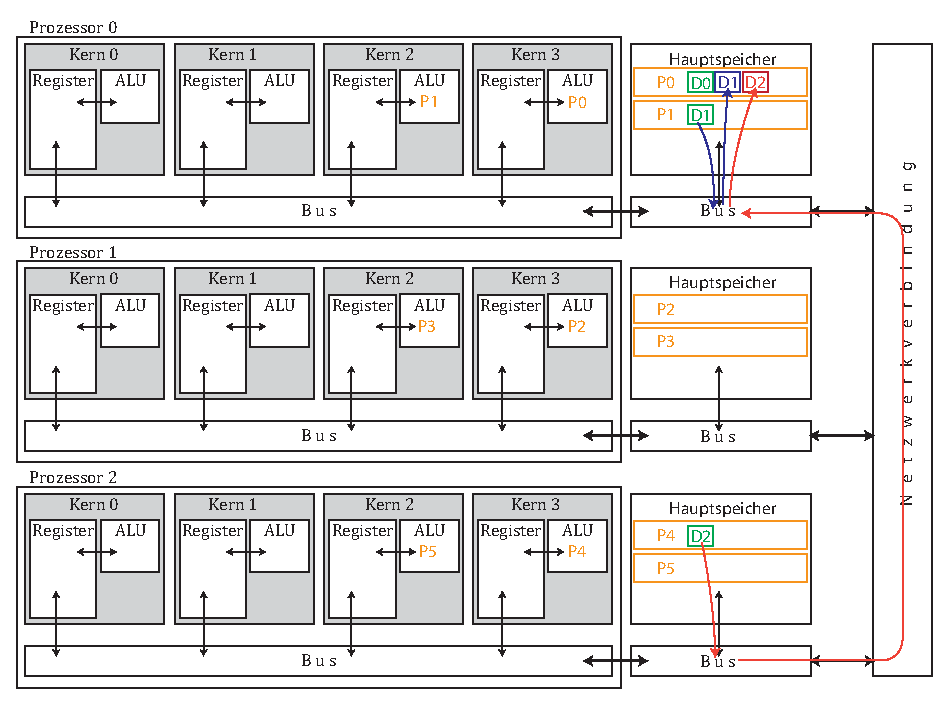
\includegraphics[width=0.9\textwidth]{img/multicorecluster_com.eps}%
% 	\caption{Eine Veranschaulichung des Message-Passings auf einem Clustersystem. In rot die Kommunikation zwischen zwei Knoten eines Clustersystems, in blau die Kommunikation innerhalb
% 	eines Knotens.}%
% 	\label{fig:message-passing}%
%       \end{figure}%
      Für unser Beispielproblem der Berechnung der Gravitationskräfte ist ein Programm vonnöten, das auf einem Clustersystem läuft und dessen Speicher verteilt verwaltet wird.
      Daher wird im folgenden Kapitel ein Parallel-Programing-Modell vorgestellt, das die Schwierigkeiten von Shared-Memory-Systemen umgeht und ein Konzept der Speicherverwaltung 
      und Kommunikation auf verteilten Rechnersystemen liefert.
      Dieses Konzept ist das sogenannte \textit{Message-Passing-Modell}. 
      Dieses Modell geht von einer Menge von \textit{autonomen} Prozessen aus, die
      \begin{enumerate}
       \item eindeutig benannt sind und
       \item jeweils über \textit{privaten Speicher} verfügen.
      \end{enumerate}
      Dies spezifiziert nicht, um welche Art Rechner(system) es sich handelt. Bei gemeinsam genutztem Hauptspeicher wird davon ausgegangen, dass jeder Prozess einen eigenen privaten 
      Bereich zugewiesen bekommt.
      
      Um nun Daten von einem Prozess $P_i$ an einen Prozess $P_j$ zu senden, muss $P_i$ explizit im Programmlauf seine Daten in Form einer Nachricht (engl.: message) verschiocken, und
      respektive $P_j$ diese Nachricht und damit die Daten in Empfang nehmen. 
%       \autoref{fig:message-passing} veranschaulicht die Wege der Nachrichten. Dabei bezeichnen $P_0,\dots,P_n$ die Prozesse und $D_0,\dots,D_2$ zugehörige Daten im Hauptspeicher. 
      
      Ein Nachteil des Message-Passing-Modells besteht in der Grundannahme von nicht gemeinsam genutztem Speicher.
      Jeder Prozess hat seine eigenen Kopien der benötigten Daten und Ergebnisse müssen explizit durch Nachrichten mitgeteilt und in die Speicherbereiche der anderen Prozesse kopiert werden. Dies
      macht das Programm aber auch weniger anfällig für Race-Conditions. Weitere Vorteile des Message-Passing-Modells sind:
      \begin{labeling}{Universalität }
	\item[Portabilität] Message-Passing ist spätestens seit \nameref{sec:mpi} (vgl.: \autoref{sec:mpi}) auf den meisten parallelen Plattformen einheitlich implementiert.
	\item[Universalität] Das Message-Passing-Modell stellt nur minimale Anforderungen an die zugrundeliegende Hardware. Es funktioniert einheitlich für vernetzte Systeme mit verteiltem 
			     Speicher ebenso, wie für Shared-Memory-Systeme oder Kombinationen aus diesen.
	\item[Einfachheit] Das Modell unterstützt explizite Kontrolle über Referenzen zu Speicherzellen und erleichtert so auch Debugging.
      \end{labeling}
      Diese Vorteile machen das Message-Passing-Modell zu einem der Standard-Modelle im High-Performance-Computing.\citep{ibm_mpm, anl_mpm, fsu_mpm}
    